
В процессе отладки модели рассматривались автономные движения отдельного 
омни-колеса.


!!!!!!!!!!!!! подчистить, ссылку на начало
Заметим, что перед началом процесса редукции индекса системы диф\-фе\-рен\-ци\-аль\-но-алгебраических уравнений полной модели экипажа, реализованного
в программном обеспечении лаборатории ди\-на\-ми\-чес\-ко\-го моделирования 
Dymola~\cite{Dymola}, эта модель составляется из: а) твердого тела платформы
омни--экипажа; б) трех твердых тел -- моделей омни--колес; в) двенадцати 
твердых тел роликов, размещенных на колесах. В соответствии, например, 
с~\cite{Kosenko2007} для каждого объекта, моделирующего твердое тело, 
реализуются шесть обыкновенных дифференциальных уравнений (ОДУ) Ньютона для
движения центра масс тела плюс семь ОДУ Эйлера для вращательного движения тела
вокруг центра масс. В последнем случае имеется четыре кинематических уравнения
Эйлера для кватерниона ориентации тела плюс три динамических уравнения Эйлера
для вектора угловой скорости твердого тела. В результате полная модель экипажа
задается системой ОДУ порядка $16\cdot 13=208$. Кроме этого, объекты 
механических связей могут генерировать дополнительные дифференциальные 
уравнения.

\begin{figure}[htb]
\centerline{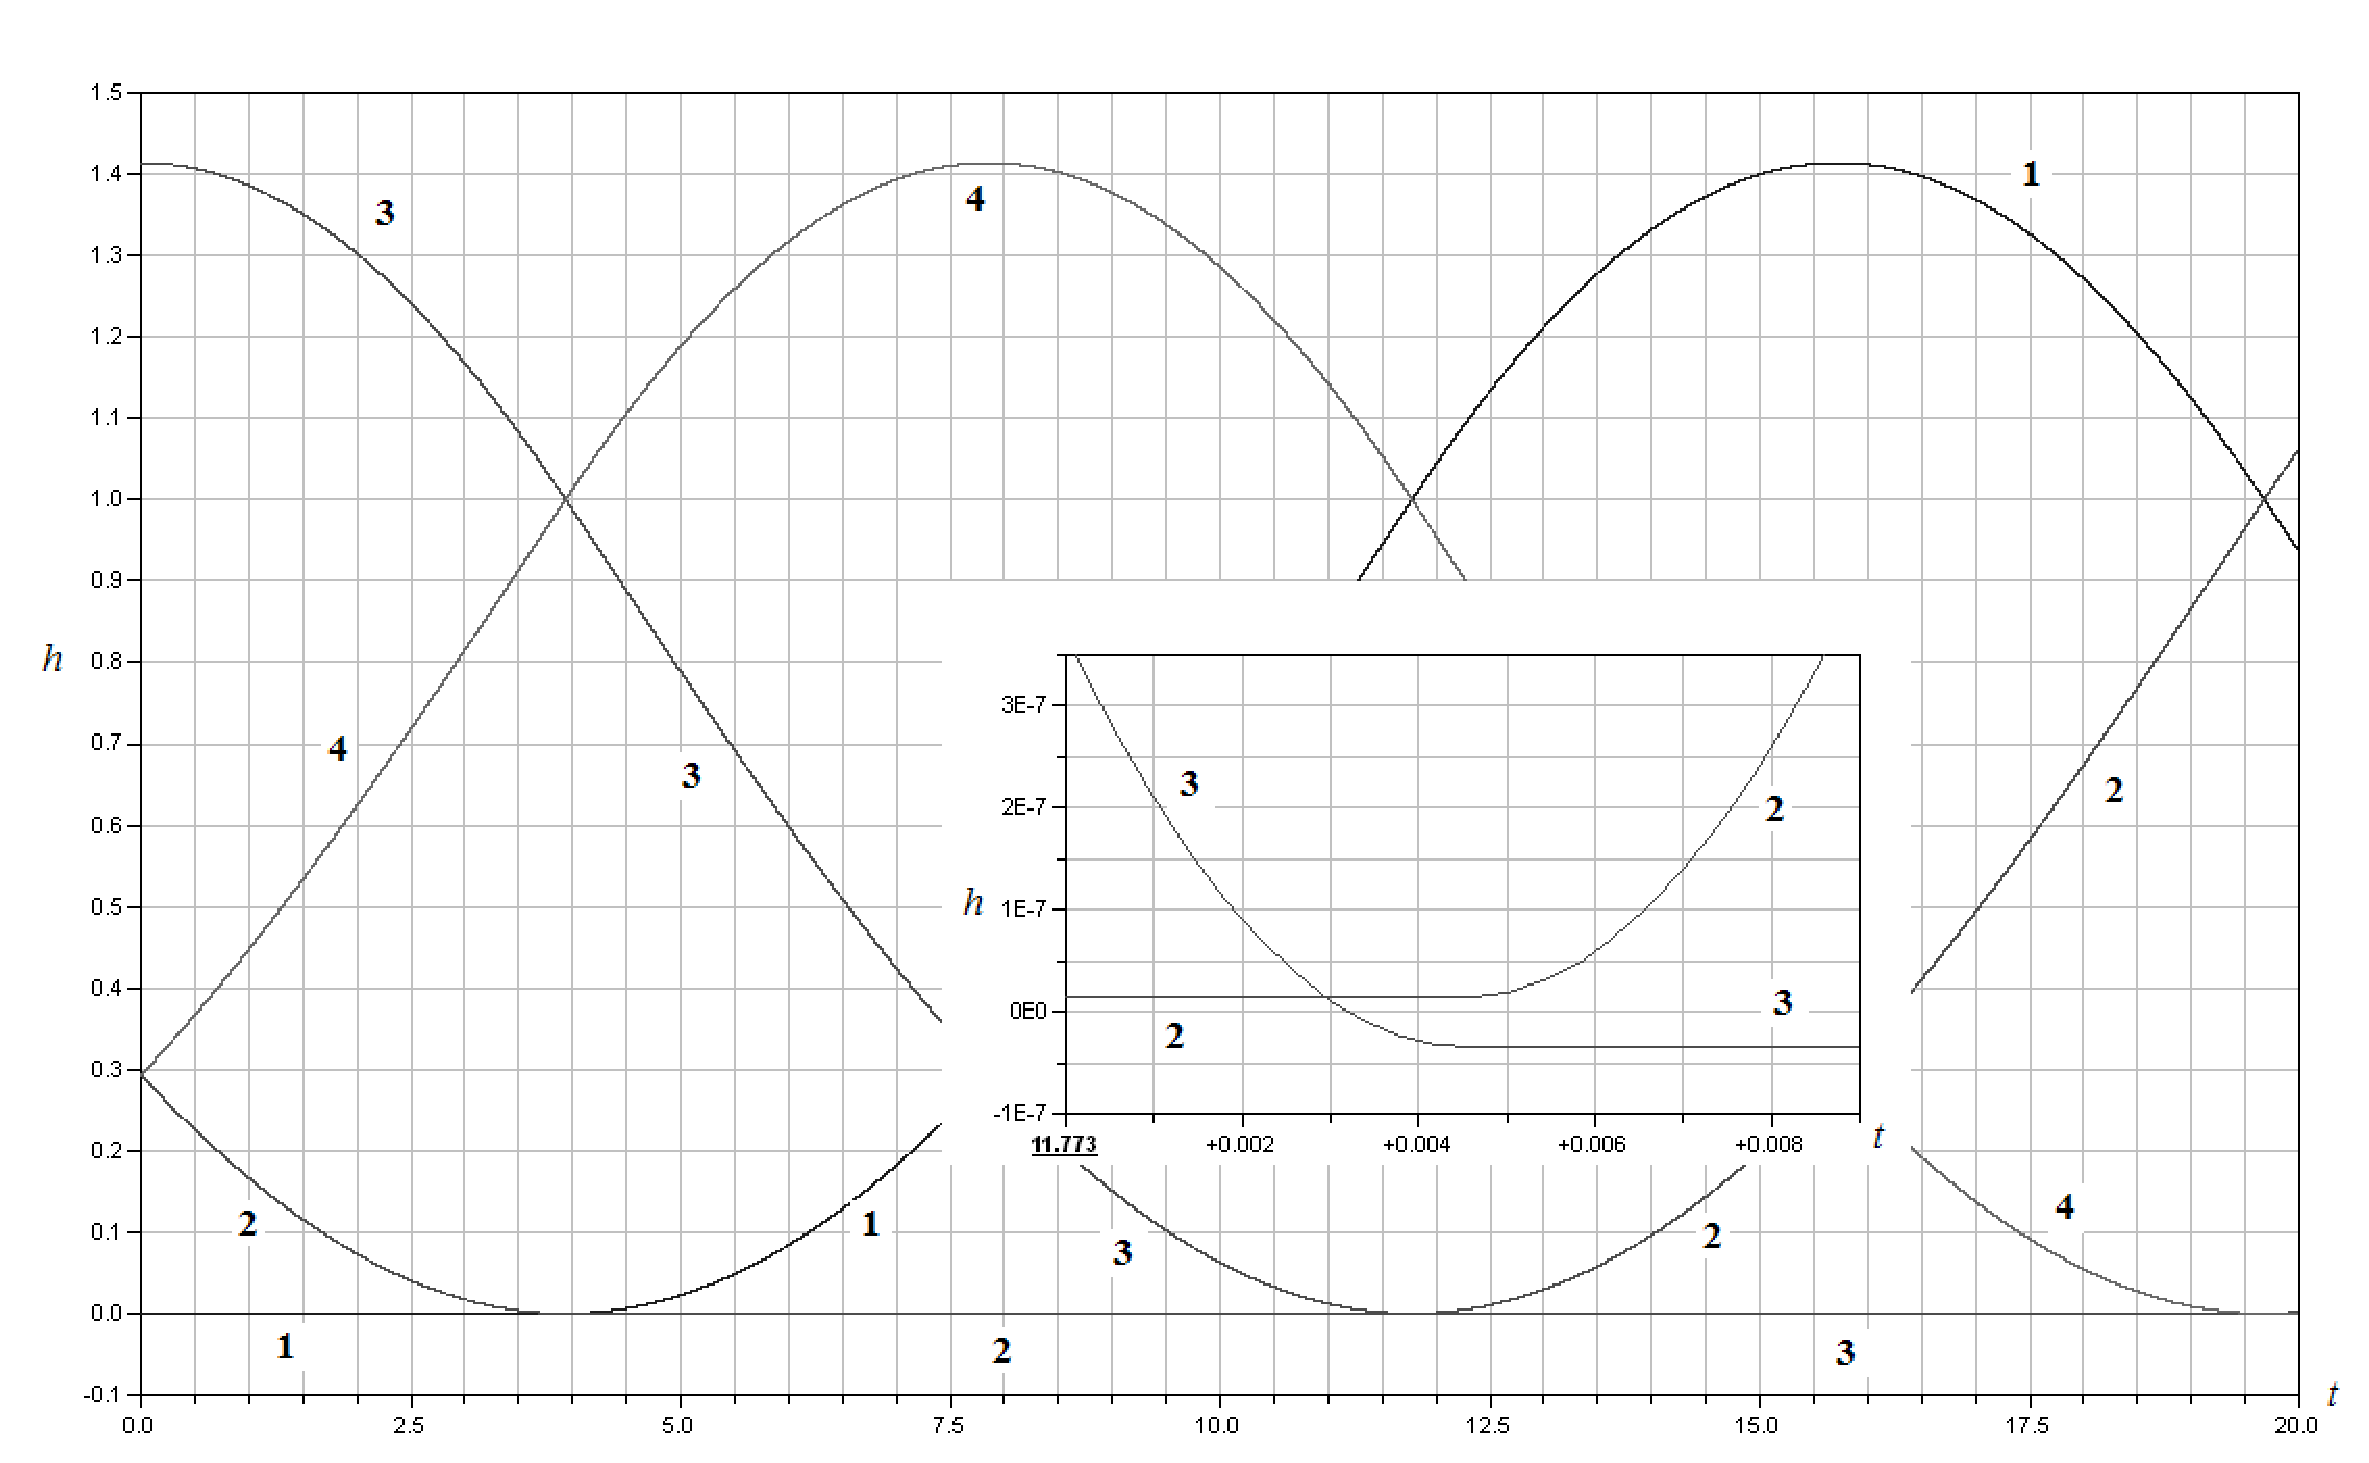
\includegraphics[width=15cm]{content/parts/3_friction/nd/Figure11.eps}}
\caption{Процесс смены роликов в контакте в численной модели.}
\label{fig1}
\end{figure}

Эволюция процесса контактирования для отдельного катящегося омни-колеса 
показана на Рис.~\ref{fig1}, где представлены зависимости  расстояний 
$h$ между горизонтальной плоскостью и роликами 
одного и того же колеса, находящимися в разных фазах (перед контактом, в 
контакте, после контакта). Номер кривой соответствует номеру ролика на колесе. В увеличенном масштабе показан момент безударного гладкого 
переключения поверхностей контактирования роликов и горизонтальной плоскости.

Одновременно можно наблюдать точность соблюдения неудерживающей связи 
(Рис.~\ref{fig2}). Здесь обнаруживается процесс постепенного увеличения
вычислительной ошибки -- расстояние между контактирующими телами медленно, для
каждого последующего ролика в контакте, увеличивается. В то же время, 
абсолютная величина ошибки остается пренебрежимо малой -- около $10^{-7}$
от единицы длины. 

\begin{figure}[htb]
\centerline{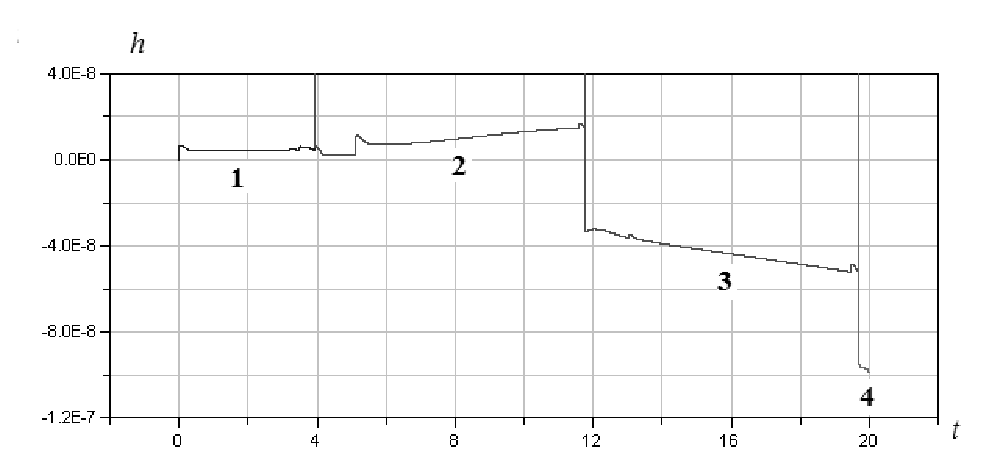
\includegraphics[width=15cm]{content/parts/3_friction/nd/Figure21.eps}}
\caption{Точность сохранения неудерживающей связи.}
\label{fig2}
\end{figure}

\section{Моделирование трения в контакте}

Конструкция омни-колеса такова, что в каждый данный 
момент времени имеется имеется только один контакт. Остальные ролики не контактируют
над полом. При этом в численном алгоритме  алгоритм отслеживания контакта продолжает 
работать, генерируя в качестве реакций нулевые усилия и моменты.

% Для каждого ролика модели омни-экипажа при контактировании  Это закон Амонтона -- Кулона
% сухого трения. На самом деле вместо этого нами используется кусочно-линейная 
% аппроксимация точного закона трения~\cite{Kosenko2006unilat}. Эта аппроксимация 
% обеспечивает высокую точность вычисления движения тел на больших интервалах 
% времени~\cite{Novozhilov1991}. 

В случае фактического выполнения контакта помимо нормальной реакции вычисляется
также её касательная составляющая, симулирующая силу трения. Для касательного 
контактного усилия имеется (как и для нормального) множество различных моделей. 
Мы остановились на реализации простейшего случая -- модели сухого трения при 
одноточечном твердотельном контакте. При этом, как известно~\cite{Novozhilov1991}, 
идеальный <<сухой>> случай реализовать не удается. Вместо разрывной функции 
sign от касательной скорости относительного скольжения контактирующих 
поверхностей используется её регуляризованный в нуле вариант. В нашем случае 
вместо функции знака sign применяется функция линейного насыщения, имеющая в 
окрестности нуля  линейный участок с большим угловым коэффициентом. Для таких функций известен 
результат~\cite{Novozhilov1991} о близости аппроксимирующего движения и движения, соответствующего <<точному>> случаю разрывной функции sign. Заметим, что и в общем случае реализация модели 
неудерживающей связи основывается на результатах, обозначенных в 
работе~\cite{Kosenko2006unilat}.

!!!!!!!!!!!!!!   Утащить после геометрии !!!!!
В данной главе описаны модели,  использующие следующие законы трения:

\begin{itemize}
    \item {
        Вязкое трение
        $$
            \vec{F}_{\text{тр}} = -\gamma\vec{v}_{C_i}
        $$
    }
    \item {
        Регуляризованное по Новожилову \cite{} сухое трение
        $$
            \vec{F}_{\text{тр}} = -\mu N \vec{v}_{C_i}
                \left\{
                    \begin{array}{ll}
                        \ddfrac{1}{\delta}, \enspace |\vec{v}_{C_i}| < \delta \ll 1 \vspace{7pt}\\
                        \ddfrac{1}{|\vec{v}_{C_i}|}\enspace \text{иначе}
                    \end{array}
                \right.
        $$
    }
\end{itemize}

Таким образом, система голономна, но ее связи не идеалны. Количество степеней свободы:
$$ 3 + N(n + 1).$$